
\section*{Aufgabe 1 -- Lineare Algebra -- 8 Punkte}

\begin{itemize}
\item [a)] $\mathbf{A} \cdot \mathbf{B} = \begin{pmatrix} 2 & 1 \\ 0 & 3 \end{pmatrix} \begin{pmatrix} 1 & -1 \\ 2 & 0 \end{pmatrix} = \begin{pmatrix} 2 \cdot 1 + 1 \cdot 2 & 2 \cdot (-1) + 1 \cdot 0 \\ 0 \cdot 1 + 3 \cdot 2 & 0 \cdot (-1) + 3 \cdot 0 \end{pmatrix} = \begin{pmatrix} 4 & -2 \\ 6 & 0 \end{pmatrix}$ (2 Punkte)
\end{itemize}

\begin{itemize}
\item [b)] $\mathbf{A}^T = \begin{pmatrix} 2 & 0 \\ 1 & 3 \end{pmatrix}$ (2 Punkte)
\end{itemize}

\begin{itemize}
\item [c)] Eine $2 \times 2$ Gewichtsmatrix verbindet 2 Eingaben (Spalten) mit 2 Ausgängen/Neuronen (Zeilen). Jedes Element $w_{ij}$ beschreibt das Gewicht zwischen Eingang $j$ und Neuron $i$. Die Matrix-Vektor-Multiplikation $\mathbf{y} = \mathbf{W} \mathbf{x}$ berechnet die gewichteten Summen für alle Neuronen gleichzeitig. (4 Punkte)
\end{itemize}

\newpage

\section*{Aufgabe 2 -- Aktivierungsfunktionen -- 7 Punkte}

\begin{itemize}
\item [a)] Sigmoid: $\sigma(x) = \frac{1}{1 + e^{-x}}$

Ableitung mit Quotientenregel:
\begin{align}
\sigma'(x) &= \frac{d}{dx}\left(\frac{1}{1 + e^{-x}}\right) \\
&= \frac{0 \cdot (1 + e^{-x}) - 1 \cdot (-e^{-x})}{(1 + e^{-x})^2} \\
&= \frac{e^{-x}}{(1 + e^{-x})^2} \\
&= \frac{1}{1 + e^{-x}} \cdot \frac{e^{-x}}{1 + e^{-x}} \\
&= \sigma(x)(1 - \sigma(x))
\end{align}
(3 Punkte)
\end{itemize}

\begin{itemize}
\item [b)] $\sigma(0) = \frac{1}{1 + e^{0}} = \frac{1}{1 + 1} = \frac{1}{2} = 0.5$ (2 Punkte)
\end{itemize}

\begin{itemize}
\item [c)] ReLU-Ableitung:
\[
\text{ReLU}'(x) = \begin{cases} 0 & \text{für } x < 0 \\ 1 & \text{für } x > 0 \end{cases}
\]
(2 Punkte)
\end{itemize}

\newpage

\section*{Aufgabe 3 -- Das Perceptron und das XOR-Problem -- 8 Punkte}

\begin{itemize}
\item [a)] Single-Layer-Perceptron mit 2 Eingängen und 1 Ausgang:
\begin{center}
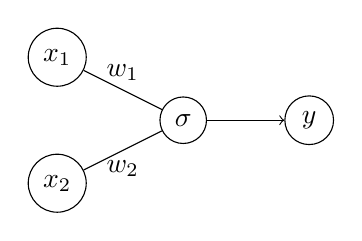
\begin{tikzpicture}[scale=0.8]
  \node[circle, draw] (x1) at (0, 1) {$x_1$};
  \node[circle, draw] (x2) at (0, -1) {$x_2$};
  \node[circle, draw] (neuron) at (2, 0) {$\sigma$};
  \node[circle, draw] (y) at (4, 0) {$y$};
  
  \draw[-] (x1) -- (neuron) node[midway, above] {$w_1$};
  \draw[-] (x2) -- (neuron) node[midway, below] {$w_2$};
  \draw[->] (neuron) -- (y);
\end{tikzpicture}
\end{center}
(2 Punkte)
\end{itemize}

\begin{itemize}
\item [b)] Ein Single-Layer-Perceptron kann nur linear separierbare Probleme lösen. Das XOR-Problem ist nicht linear separierbar: Es gibt keine einzelne Gerade, die die zwei Klassen (XOR=0 und XOR=1) voneinander trennen kann. (2 Punkte)
\end{itemize}

\begin{itemize}
\item [c)] Multi-Layer-Perceptron:
\begin{center}
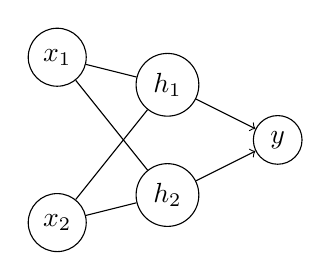
\begin{tikzpicture}[scale=0.7]
  \node[circle, draw] (x1) at (0, 1.5) {$x_1$};
  \node[circle, draw] (x2) at (0, -1.5) {$x_2$};
  \node[circle, draw] (h1) at (2, 1) {$h_1$};
  \node[circle, draw] (h2) at (2, -1) {$h_2$};
  \node[circle, draw] (y) at (4, 0) {$y$};
  
  \draw[-] (x1) -- (h1);
  \draw[-] (x1) -- (h2);
  \draw[-] (x2) -- (h1);
  \draw[-] (x2) -- (h2);
  \draw[->] (h1) -- (y);
  \draw[->] (h2) -- (y);
\end{tikzpicture}
\end{center}

Anzahl der Gewichte: $2 \times 2 = 4$ Gewichte (Input→Hidden) + $2 \times 1 = 2$ Gewichte (Hidden→Output) + 2 Biases (Hidden) + 1 Bias (Output) = **9 Parameter** (oder nur Gewichte: 6) (2 Punkte)
\end{itemize}

\begin{itemize}
\item [d)] Das tiefere Netzwerk mit Hidden Layer kann nicht-lineare Funktionen durch die Aktivierungsfunktion (ReLU/Sigmoid) kombinieren. Der Hidden Layer transformiert die Eingaben in einen neuen Raum, wo XOR linear separierbar wird. (2 Punkte)
\end{itemize}

\newpage

\section*{Aufgabe 4 -- Partielle Ableitungen und Kettenregel -- 9 Punkte}

\begin{itemize}
\item [a)] $\frac{\partial L}{\partial a} = \frac{\partial}{\partial a}\left[\frac{1}{2}(y-a)^2\right] = \frac{1}{2} \cdot 2(y-a) \cdot (-1) = -(y-a) = a - y$ (1 Punkt)
\end{itemize}

\begin{itemize}
\item [b)] $\frac{\partial a}{\partial z} = \frac{\partial \sigma(z)}{\partial z} = \sigma(z)(1-\sigma(z))$ (1 Punkt)
\end{itemize}

\begin{itemize}
\item [c)] $\frac{\partial z}{\partial w} = \frac{\partial(w \cdot x + b)}{\partial w} = x$ (1 Punkt)
\end{itemize}

\begin{itemize}
\item [d)] $\frac{\partial L}{\partial w} = \frac{\partial L}{\partial a} \cdot \frac{\partial a}{\partial z} \cdot \frac{\partial z}{\partial w} = (a-y) \cdot \sigma(z)(1-\sigma(z)) \cdot x$ (2 Punkte)
\end{itemize}

\begin{itemize}
\item [e)] Gegeben: $x=1, w=0.5, b=0, y=1, \sigma(0.5) \approx 0.62$

$z = 0.5 \cdot 1 + 0 = 0.5$ (0.5 Punkte)

$a = \sigma(0.5) \approx 0.62$ (0.5 Punkte)

$\sigma(0.5) \cdot (1 - \sigma(0.5)) \approx 0.62 \cdot 0.38 \approx 0.236$ (1 Punkt)

$\frac{\partial L}{\partial w} = (0.62 - 1) \cdot 0.236 \cdot 1 = (-0.38) \cdot 0.236 \approx -0.090$ (1 Punkt)
\end{itemize}

\newpage

\section*{Aufgabe 5 -- Forward Pass eines 2-Schicht-Netzwerks -- 9 Punkte}

\begin{itemize}
\item [a)] $\mathbf{z}^H = \begin{pmatrix} 0.5 & 0.3 \\ 0.2 & 0.4 \end{pmatrix} \begin{pmatrix} 1 \\ 1 \end{pmatrix} + \begin{pmatrix} 0 \\ 0 \end{pmatrix} = \begin{pmatrix} 0.8 \\ 0.6 \end{pmatrix}$ (1 Punkt)
\end{itemize}

\begin{itemize}
\item [b)] $\mathbf{a}^H = \text{ReLU}(\mathbf{z}^H) = \text{ReLU}\begin{pmatrix} 0.8 \\ 0.6 \end{pmatrix} = \begin{pmatrix} 0.8 \\ 0.6 \end{pmatrix}$ (beide positiv) (1 Punkt)
\end{itemize}

\begin{itemize}
\item [c)] $\hat{y} = \begin{pmatrix} 1 & 1 \end{pmatrix} \begin{pmatrix} 0.8 \\ 0.6 \end{pmatrix} + 0 = 1 \cdot 0.8 + 1 \cdot 0.6 = 1.4$ (1.5 Punkte)
\end{itemize}

\begin{itemize}
\item [d)] $L = \frac{1}{2}(2 - 1.4)^2 = \frac{1}{2}(0.6)^2 = \frac{1}{2} \cdot 0.36 = 0.18$ (1.5 Punkte)
\end{itemize}

\begin{itemize}
\item [e)] $\frac{\partial L}{\partial \hat{y}} = -(y - \hat{y}) = -(2 - 1.4) = -0.6$ (1 Punkt)
\end{itemize}

\begin{itemize}
\item [f)] $\frac{\partial L}{\partial w_1^O} = \frac{\partial L}{\partial \hat{y}} \cdot \frac{\partial \hat{y}}{\partial w_1^O} = -0.6 \cdot a_1^H = -0.6 \cdot 0.8 = -0.48$ (1.5 Punkte)
\end{itemize}

\newpage

\section*{Aufgabe 6 -- Gradient Descent -- 7 Punkte}

\begin{itemize}
\item [a)] Gewichtsaktualisierungsformel:
\[
w_{\text{neu}} = w_{\text{alt}} - \eta \frac{\partial L}{\partial w}
\]
wobei $\eta$ die Learning Rate ist. (1.5 Punkte)
\end{itemize}

\begin{itemize}
\item [b)] $w_{\text{neu}} = 0.5 - 0.1 \cdot 0.4 = 0.5 - 0.04 = 0.46$ (1.5 Punkte)
\end{itemize}

\begin{itemize}
\item [c)] Zwei Probleme bei zu hoher Learning Rate:
\begin{itemize}
  \item Divergenz: Die Gewichte können zu weit wandern und den Optimalen Punkt überschießen
  \item Oscillation: Der Algorithmus springt hin und her, statt zu konvergieren
\end{itemize}
(2 Punkte)
\end{itemize}

\begin{itemize}
\item [d)] 
\begin{itemize}
  \item \textbf{Batch GD}: Verwendet alle Daten pro Update (stabiler, aber langsamer)
  \item \textbf{SGD}: Verwendet eine zufällige Probe pro Update (schneller, aber rauschiger)
\end{itemize}
(2 Punkte)
\end{itemize}

\newpage

\section*{Aufgabe 7 -- Convolutional Neural Networks (CNNs) -- 8 Punkte}

\begin{itemize}
\item [a)] Zwei Gründe:
\begin{itemize}
  \item \textbf{Räumliche Struktur}: Convolution nutzt lokale räumliche Muster (Filter) statt globaler Features
  \item \textbf{Parameter-Reduktion}: Gleicher Filter wird überall angewendet → viel weniger Parameter als vollverbundenes Netz
\end{itemize}
(2 Punkte)
\end{itemize}

\begin{itemize}
\item [b)] Die Convolution-Operation: Ein Filter (Kernel) wird über das Bild gefahren. An jeder Position wird das Element-weise Produkt des Filters mit der lokalen Bildregion berechnet und summiert. Dies erkennt lokale Muster wie Kanten, Ecken, etc. (2 Punkte)
\end{itemize}

\begin{itemize}
\item [c)] Max-Pooling $2 \times 2$ auf $4 \times 4$ Feature Map:

Eingabe: $\begin{pmatrix} 1 & 2 & 3 & 4 \\ 5 & 6 & 7 & 8 \\ 9 & 10 & 11 & 12 \\ 13 & 14 & 15 & 16 \end{pmatrix}$

Ausgabe: $\begin{pmatrix} 6 & 8 \\ 14 & 16 \end{pmatrix}$ (Max-Pooling nimmt das Maximum aus jedem $2 \times 2$ Block)

(2 Punkte)
\end{itemize}

\begin{itemize}
\item [d)] Zwei CNN-Architekturen:
\begin{itemize}
  \item \textbf{LeNet-5}: Frühe CNN, 5-7 Layer, gut für MNIST
  \item \textbf{ResNet}: Mit Skip-Connections, ermöglicht sehr tiefe Netze (50+ Layer)
  \item \textbf{VGG}: Einfache Architektur mit kleinen $3 \times 3$ Filtern, sehr beliebt
\end{itemize}
(2 Punkte - eine beliebige Architektur mit Besonderheit)
\end{itemize}

\newpage

\section*{Aufgabe 8 -- RNNs und LSTMs -- 8 Punkte}

\begin{itemize}
\item [a)] Zwei Gründe:
\begin{itemize}
  \item \textbf{Sequenzgedächtnis}: RNN hat versteckten State $h_t$, der Information über vorherige Zeitschritte trägt
  \item \textbf{Temporale Abhängigkeiten}: Vollverbundene Netze ignorieren die zeitliche Struktur, RNNs modellieren sie
\end{itemize}
(2 Punkte)
\end{itemize}

\begin{itemize}
\item [b)] Das Vanishing Gradient Problem: Bei Backpropagation through Time (BPTT) werden Gradienten exponentiell klein, wenn man mehrere Zeitschritte zurückgeht. Dies verhindert, dass das Netz von weit entfernten Zeitschritten lernt. (2 Punkte)
\end{itemize}

\begin{itemize}
\item [c)] LSTM-Zelle mit vier Komponenten:
\begin{center}
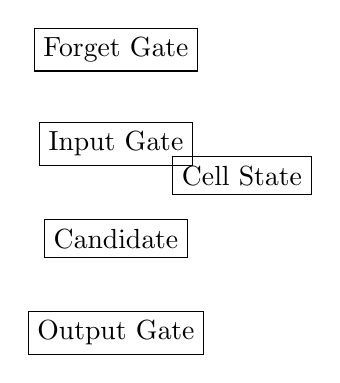
\begin{tikzpicture}[scale=0.8]
  \node[rectangle, draw] at (0, 2) {Forget Gate};
  \node[rectangle, draw] at (0, 0.5) {Input Gate};
  \node[rectangle, draw] at (0, -1) {Candidate};
  \node[rectangle, draw] at (0, -2.5) {Output Gate};
  \node[rectangle, draw] at (2, 0) {Cell State};
\end{tikzpicture}
\end{center}
Forget Gate kontrolliert, welche alte Info gelöscht wird; Input Gate, was neue Info hinzugefügt wird; Candidate ist neue Info; Output Gate kontrolliert Output. (2 Punkte)
\end{itemize}

\begin{itemize}
\item [d)] LSTMs lösen das Problem durch die Cell State (Zellzustand), die durch Multiplikation (nicht Kettenregel) von Forget Gate mit altem State aktualisiert wird. Dies erlaubt, dass Gradienten direkt durch die Cell State fließen, ohne exponentiell zu schrumpfen. (2 Punkte)
\end{itemize}

\newpage

\section*{Aufgabe 9 -- Generative Modelle -- 7 Punkte}

\begin{itemize}
\item [a)] 
\begin{itemize}
  \item \textbf{Diskriminative Modelle}: Lernen $P(y|x)$ - Klassifikation/Regression von Input zu Label. Beispiel: CNN für Bildklassifikation
  \item \textbf{Generative Modelle}: Lernen $P(x)$ oder $P(x,y)$ - können neue Daten generieren. Beispiel: GAN für Bildgenerierung
\end{itemize}
(2 Punkte)
\end{itemize}

\begin{itemize}
\item [b)] GAN-Architektur:
\begin{center}
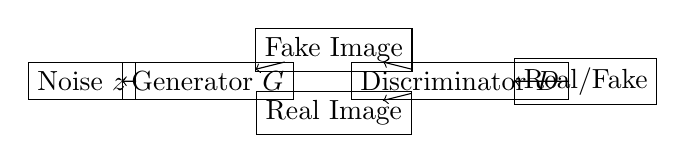
\begin{tikzpicture}[scale=0.8]
  \node[rectangle, draw] (noise) at (0, 1) {Noise $z$};
  \node[rectangle, draw] (gen) at (2, 1) {Generator $G$};
  \node[rectangle, draw] (fake) at (4, 1.5) {Fake Image};
  \node[rectangle, draw] (real) at (4, 0.5) {Real Image};
  \node[rectangle, draw] (disc) at (6, 1) {Discriminator $D$};
  \node[rectangle, draw] (out) at (8, 1) {Real/Fake};
  
  \draw[->] (noise) -- (gen);
  \draw[->] (gen) -- (fake);
  \draw[->] (fake) -- (disc);
  \draw[->] (real) -- (disc);
  \draw[->] (disc) -- (out);
\end{tikzpicture}
\end{center}
Generator erzeugt Fake-Bilder; Discriminator unterscheidet Real von Fake. (2.5 Punkte)
\end{itemize}

\begin{itemize}
\item [c)] Zwei Anwendungen:
\begin{itemize}
  \item Bildgenerierung (Gesichter, Kunstwerke)
  \item Bild-zu-Bild-Translation (Style Transfer, Datensatzerweiterung)
  \item Text-zu-Bild-Generierung
\end{itemize}
(2.5 Punkte)
\end{itemize}

\newpage

\section*{Aufgabe 10 -- Overfitting und Regularisierung -- 7 Punkte}

\begin{itemize}
\item [a)] 

\textbf{Underfitting} (zu einfaches Modell): Training-Loss und Validation-Loss sind beide hoch.

\textbf{Good Fit}: Training-Loss sinkt, Validation-Loss sinkt ähnlich, beide Kurven sind nah beieinander.

\textbf{Overfitting} (zu komplexes Modell): Training-Loss sinkt sehr niedrig, Validation-Loss beginnt zu steigen.

\begin{center}
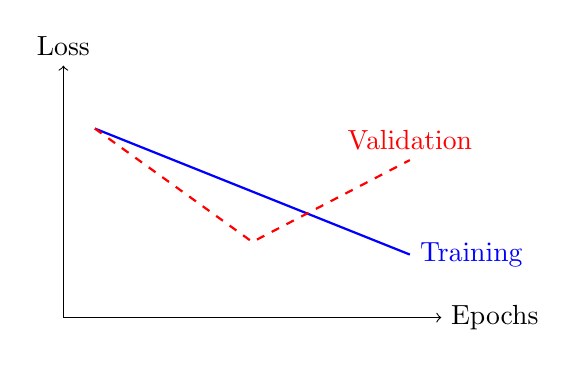
\begin{tikzpicture}[scale=0.8]
  \draw[->] (0,0) -- (6,0) node[right] {Epochs};
  \draw[->] (0,0) -- (0,4) node[above] {Loss};
  
  \draw[blue, thick] (0.5,3) -- (5.5,1) node[right] {Training};
  \draw[red, dashed, thick] (0.5,3) -- (3,1.2) -- (5.5,2.5) node[above] {Validation};
\end{tikzpicture}
\end{center}
(3 Punkte)
\end{itemize}

\begin{itemize}
\item [b)] Drei Techniken zur Vermeidung von Overfitting:
\begin{itemize}
  \item \textbf{Dropout}: Zufällig Neuronen während Training deaktivieren
  \item \textbf{Regularisierung} (L1/L2): Gewichte bestrafen im Loss
  \item \textbf{Early Stopping}: Training stoppen, wenn Validation-Loss steigt
  \item \textbf{Data Augmentation}: Mehr Trainingsdaten erstellen
\end{itemize}
(2 Punkte - mindestens 3)
\end{itemize}

\begin{itemize}
\item [c)] Dropout: Während Training werden zufällig mit Wahrscheinlichkeit $p$ (typisch 0.5) Neuronen auf 0 gesetzt. Dies erzwingt, dass das Netz redundante Features nicht verlässlich nutzen kann. (2 Punkte)
\end{itemize}

\begin{itemize}
\item [d)] Bei Inferenz wird Dropout deaktiviert oder die Ausgaben um $(1-p)$ skaliert, um den veränderten Durchschnitt zu korrigieren. Dies stellt sicher, dass die erwartete Aktivierung gleich bleibt. (2 Punkte)
\end{itemize}

\newpage

\section*{Aufgabe 11 -- Gradienten in Vektorform -- 8 Punkte}

\begin{itemize}
\item [a)] $\frac{\partial L}{\partial \hat{y}} = -(y - \hat{y}) = \hat{y} - y$ (1 Punkt)
\end{itemize}

\begin{itemize}
\item [b)] $\frac{\partial \hat{y}}{\partial \mathbf{w}} = \mathbf{a}$ (der Vektor der Hidden-Ausgaben) (1 Punkt)
\end{itemize}

\begin{itemize}
\item [c)] $\frac{\partial L}{\partial \mathbf{w}} = \frac{\partial L}{\partial \hat{y}} \cdot \frac{\partial \hat{y}}{\partial \mathbf{w}} = (\hat{y} - y) \cdot \mathbf{a}$ (2 Punkte)
\end{itemize}

\begin{itemize}
\item [d)] $\frac{\partial L}{\partial \mathbf{w}} = (0.75 - 2) \cdot \begin{pmatrix} 1 \\ 0.5 \end{pmatrix} = (-1.25) \cdot \begin{pmatrix} 1 \\ 0.5 \end{pmatrix} = \begin{pmatrix} -1.25 \\ -0.625 \end{pmatrix}$ (2 Punkte)
\end{itemize}

\begin{itemize}
\item [e)] Der Gradient $\nabla L = \frac{\partial L}{\partial \mathbf{w}}$ zeigt in die Richtung des steilsten Anstiegs des Verlusts. Für Minimierung müssen wir in die entgegengesetzte Richtung gehen: $\mathbf{w}_{\text{neu}} = \mathbf{w}_{\text{alt}} - \eta \nabla L$. Das Minuszeichen ist crucial für das Funktionieren von Gradient Descent. (2 Punkte)
\end{itemize}

\newpage

\section*{Aufgabe 12 -- Momentum und adaptive Learning Rates -- 8 Punkte}

\begin{itemize}
\item [a)] Momentum-Methode: Der Gradient wird nicht direkt angewendet, sondern mit einem "Impuls" $v$ kombiniert:
\begin{align}
v_t &= \beta v_{t-1} + \frac{\partial L}{\partial w} \\
w_{t+1} &= w_t - \eta v_t
\end{align}
wobei $\beta \approx 0.9$ die Momentum-Konstante ist. Dies addiert Trägheit und hilft, lokale Minima zu überwinden. (2 Punkte)
\end{itemize}

\begin{itemize}
\item [b)] 
\begin{itemize}
  \item \textbf{SGD}: Aktualisiert direkt mit Gradienten, keine Trägheit
  \item \textbf{Momentum}: Nutzt exponentiell gewichtete Durchschnitte von Gradienten für schnellere Konvergenz und bessere Beschleunigung
\end{itemize}
(1.5 Punkte)
\end{itemize}

\begin{itemize}
\item [c)] ADAM (Adaptive Moment Estimation):
\begin{align}
m_t &= \beta_1 m_{t-1} + (1-\beta_1) \frac{\partial L}{\partial w} & \text{(erstes Moment)} \\
v_t &= \beta_2 v_{t-1} + (1-\beta_2) \left(\frac{\partial L}{\partial w}\right)^2 & \text{(zweites Moment)} \\
w_{t+1} &= w_t - \eta \frac{m_t}{\sqrt{v_t} + \epsilon}
\end{align}
Parameter: $\beta_1 \approx 0.9$, $\beta_2 \approx 0.999$, $\eta \approx 0.001$, $\epsilon = 10^{-8}$ (2.5 Punkte)
\end{itemize}

\begin{itemize}
\item [d)] ADAM ist besser als Standard Gradient Descent, wenn:
\begin{itemize}
  \item Sparse Gradienten (viele Nullen)
  \item Unterschiedliche Skalierung verschiedener Gewichte
  \item Non-stationäre Probleme
  \item Schnelle Konvergenz gewünscht
\end{itemize}
(1 Punkt)
\end{itemize}

\begin{itemize}
\item [e)] Der Vorteil adaptiver Learning Rates: Jeder Parameter bekommt eine individuell angepasste Learning Rate. Häufig aktualisierte Parameter bekommen kleinere Rates, selten aktualisierte bekommen größere Rates. Dies ermöglicht schnelleres Training mit einer einzigen Standard-Lernrate. (1 Punkt)
\end{itemize}
